% The first argument is the \documentclass, which tells latex which template
% we're using to build this document. It's usually safe to just use "article".
\documentclass{article}

% include some packages...
\usepackage{fullpage} % change settings for a smaller margin
\usepackage{graphicx} % gives access to the \includegraphics commands
\usepackage{amsfonts}
\usepackage{float}
\usepackage{enumitem}
\usepackage{bookmark}
\usepackage{caption}
\graphicspath{{./images/}}

% tell Latex to use no paragraph indentation, but leave some space between
% paragraphs 
\setlength{\parindent}{0in}
\setlength{\parskip}{0.1in}

\newcommand{\tib}[1]{\textit{\textbf{#1}}}
\newcommand{\code}[1]{\texttt{#1}}

% these commands merely set the values for the title/date/author; they don't put
% them in the document... see \maketitle below
\title{CS Department Automated Information Timeline. \\ Assignment 3.1: Domain Model}
\date{\today}
\author{Matthew Hays, Pawan Bhandari, Sarah Faron, Tim Klimpel}

% all document content goes between \begin{document} and \end{document}
\begin{document}

% this command actually creates the title/date/author in the document
\maketitle
\newpage
\tableofcontents
\listoffigures
\newpage

According to C. Larman, The three strategies to identify candidate concepts are reuse or modify existing models, use a category list and identify noun phrases. The concepts on the domain model for CS Department Automated Information Timeline project have been derived by identifying the noun phrases from the requirements and use cases.

\section{Concepts, Attributes, and Associations (Draft)}
Below are the candidate concepts and their attributes identified using the noun phrases from the requirements.\\

\begin{minipage}{0.3\textwidth}
    \begin{enumerate}
        \item \textbf{Post}: title, content
        \item \textbf{DisplayedPost}
        \item \textbf{Page}: title, content
        \item \textbf{Event}: dateOfEvent
        \item \textbf{EventCalender}
        \item \textbf{Media}: title, mediatype
        \item \textbf{MediaLibrary}
        \item \textbf{Notification}
        \item \textbf{Faculty}: name
        \item \textbf{OfficeManager}: name
        \item \textbf{Administrator}
        \item \textbf{DisplayedMedia}
        \item \textbf{DisplayMonitor}
    \end{enumerate}
\end{minipage}%
\begin{minipage}{0.7\textwidth}
    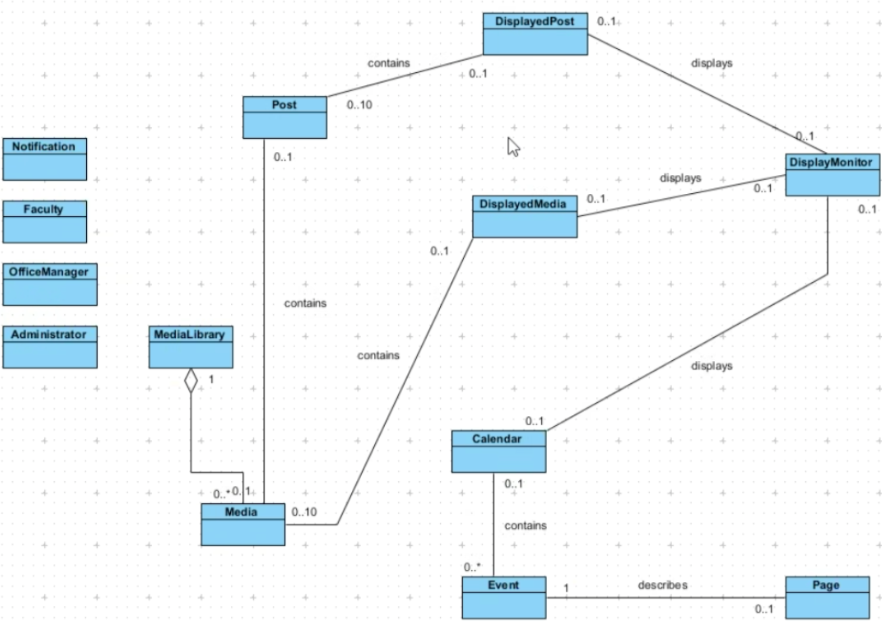
\includegraphics[scale=0.52]{images/draft-Concepts.png}
    \captionof{figure}{Candidate concepts and associations (Draft)}
\end{minipage}

These candidate concepts are further discussed among the team members and are further refined to create a final version of the domain model.

\section{Domain Model}
    \subsection{Domain Model (Draft)}
        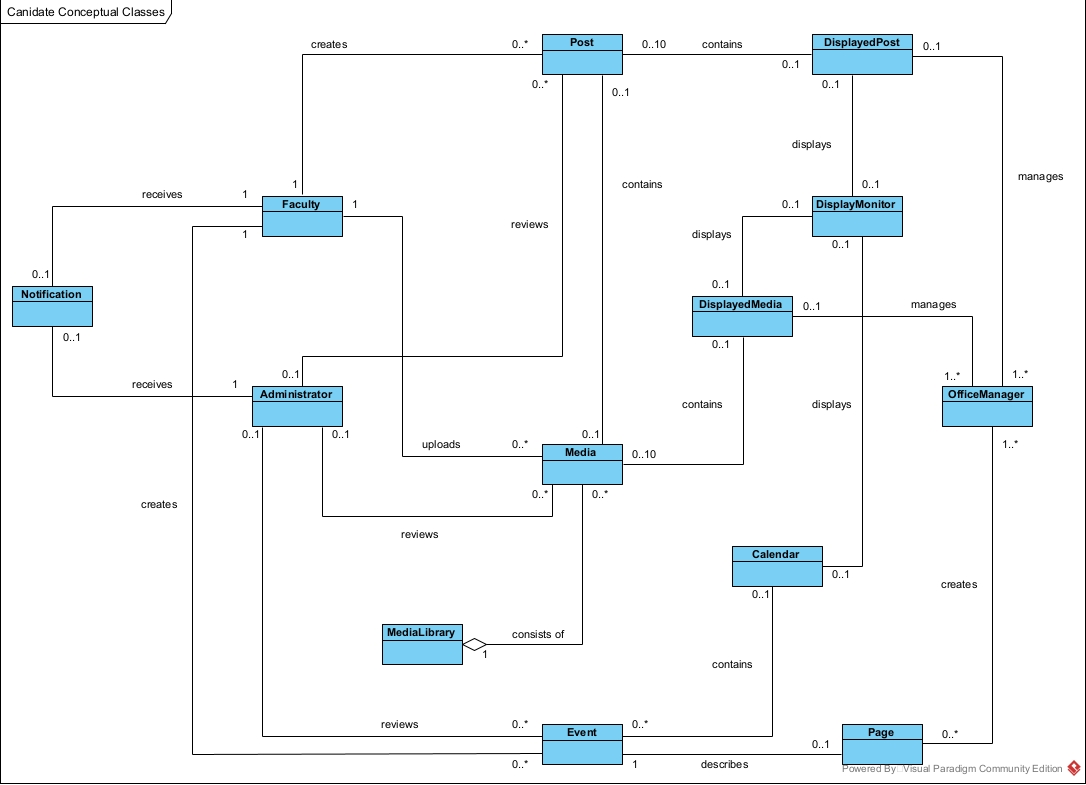
\includegraphics[scale=0.44]{images/draft-DomainModel.png}
        \captionof{figure}{Domain Model Draft}
        \label{fig:enter-label}

        
    \subsection{Discussion of domain model draft}
    TODO: What to include??\\
    Copy your draft and reason about your use cases, data you might need to collect, and any unnecessary redundancy or cycles

    
    \subsection{Domain Model (Final)}
     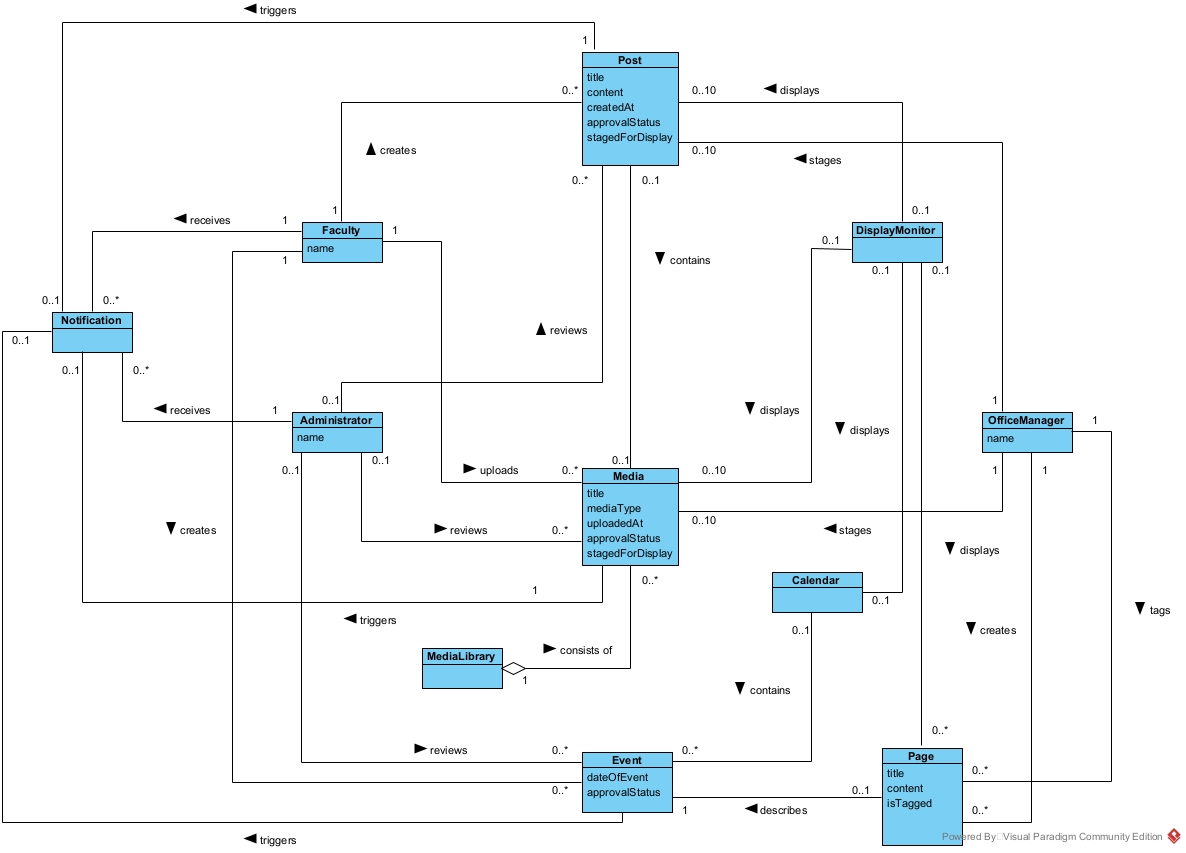
\includegraphics[scale=0.45]{images/DomainModel.jpg}
        \captionof{figure}{Final version of the Domain Model}
        \label{fig:enter-label}
        
\end{document}